% !TEX root = Simulation.tex

\chapter{Cellular Automata - Chapter 7}

\section{Problem 1 (from slides)}
\textbf{
Modify the heat flow example to deal with insulated conditions on the top and bottom boundary. Insulation means zero flux or u[N][j] = u[N-1][j]. This implies that instead of fixed valued ghost points on the top and bottom, you modify the CA rule using the previous relation.
}

\hfill \\

Assuming we were using the averaging method used in the python in the slides, I adapted it to use a No Flux condition at the top and bottom boundaries. To make the with and without runs easier to compare I ran two CAs at the same time, one without the condition and one with. In the one with the condition, the top and bottom ghost points were set to the values directly below and above them respectively after every iteration. The code can be found in Listing~\ref{HeatFlowCA.py} and the results can be seen in Figure~\ref{heatflow_results}.

\begin{figure}
\centering
\begin{tabular}{c c} 
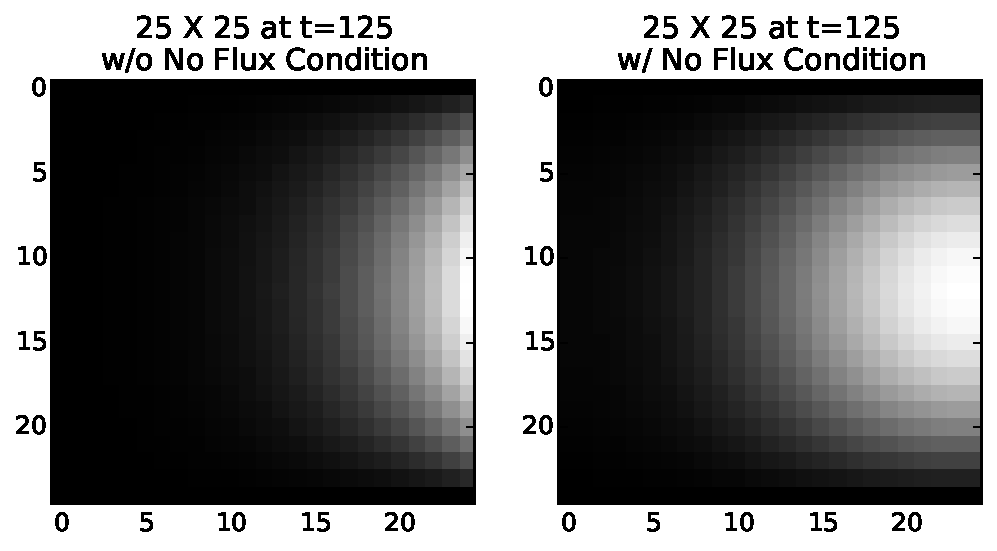
\includegraphics[width=.45\textwidth]{CAs/heatflow_25_125} & 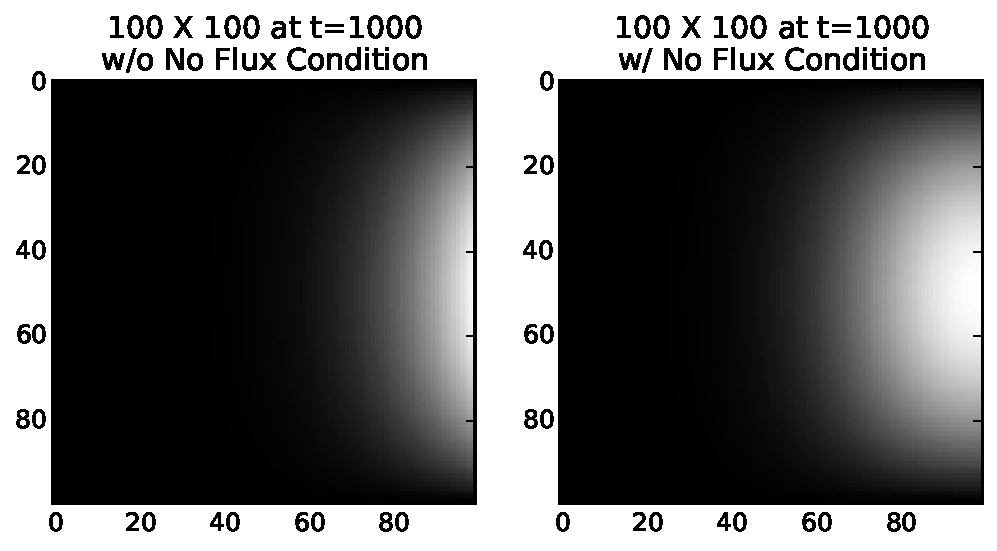
\includegraphics[width=.45\textwidth]{CAs/heatflow_100_1000} \\
(a) & (b) \\
\end{tabular}
\caption{Results for Problem 1 in the slides. (a) 25 X 25 CA after 125 iterations. (b) 100 X 100 CA after 1000 iterations}
\label{heatflow_results}
\end{figure}

\section{Problem 2 (from slides)}
\textbf{
Reproduce patterns theta, lambda, mu, and alpha in the Gray-Scott Model CA. You don't need to follow their color scheme.
}

\hfill \\

The first step here is to collect the data necessary to reproduce these patterns. Since the code was available in a couple formats, I decided to use that and gather the parameters necessary to create the patterns from the internet. I stumbled upon a good site (\url{http://mrob.com/pub/comp/xmorphia/pearson-classes.html}) with parameters available for each of the necessary patterns. Table~\ref{pattern_params} is a summary of the parameters necessary for this assignment.

The first attempt was in python and can be found in Listing~\ref{GrayScottCA.py}. The code that actually got results was in C/C++ and can be seein in Listing~\ref{GrayScott.cpp}. The final resulting patterns (plotted with gnuplot) can be seen in Figure~\ref{grayscott_results}.

\begin{figure}
\centering
\begin{tabular}{ c c }
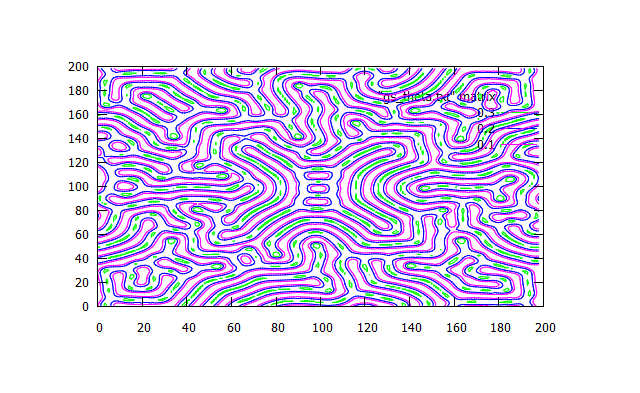
\includegraphics[width=.45\textwidth]{CAs/gs_theta} &
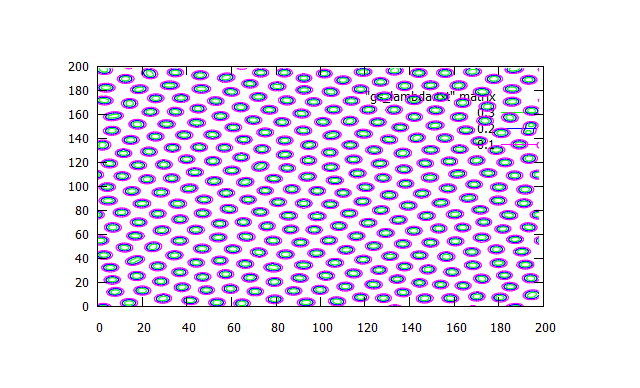
\includegraphics[width=.45\textwidth]{CAs/gs_lambda} \\
(a) & (b) \\ \\
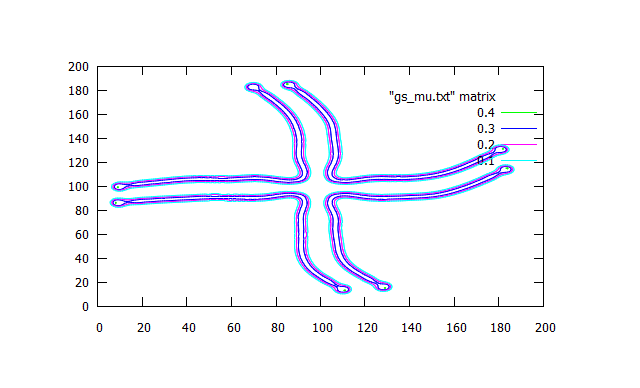
\includegraphics[width=.45\textwidth]{CAs/gs_mu} &
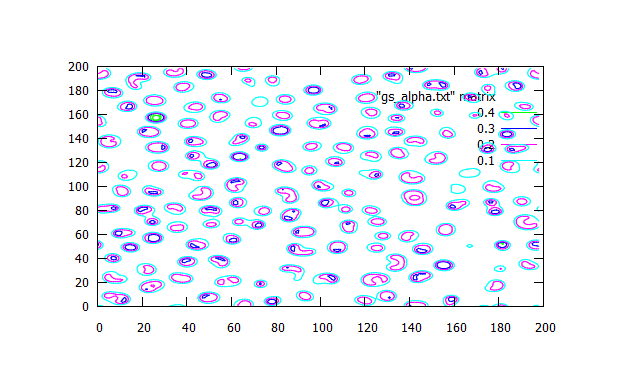
\includegraphics[width=.45\textwidth]{CAs/gs_alpha} \\
(c) & (d) \\
\end{tabular}
\caption{Results from the Gray-Scott Models: (a) Theta, (b) Lambda, (c) Mu, and (d) Alpha}
\label{grayscott_results}
\end{figure}

\begin{table}
\centering
\begin{tabular}{ r | c c }
Pattern & F & k \\
\hline
theta ($\theta$) & 0.030 & 0.057 \\
lambda ($\lambda$) & 0.026 & 0.061 \\
mu ($\mu$) & 0.046 & 0.065 \\
alpha ($\alpha$) & 0.014 & 0.053
\end{tabular}
\caption{Parameters for Gray-Scott patterns.}
\label{pattern_params}
\end{table}
